
\begin{figure}[t]
    \centering
    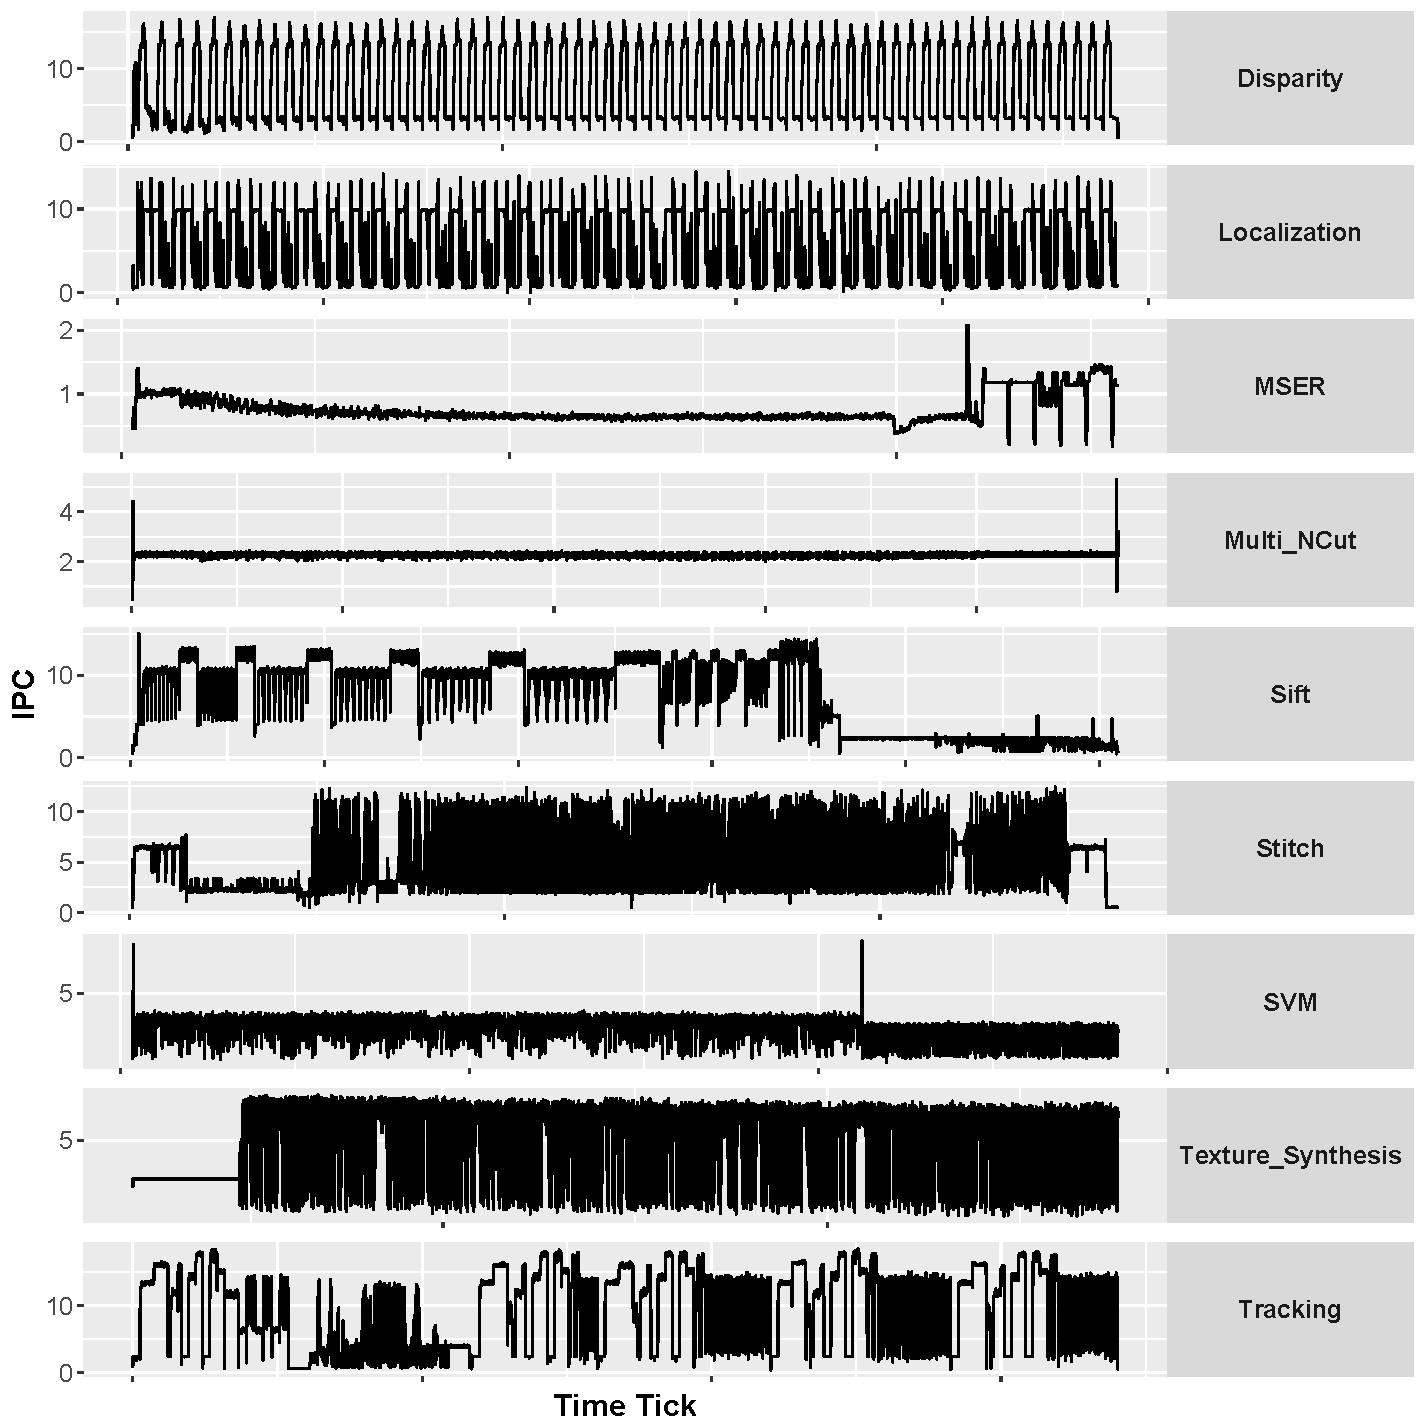
\includegraphics[width=1\textwidth]{cases-paper/graphics/Exploration/ipcs_16_3.pdf}
    \caption{IPC as a function of time for each benchmark when run on 16 fused cores.}
    \label{fig:sxt}
	\vspace{2em}
\end{figure}

This section explores how core composition affects the performance of the SD-VBS benchmarks.
First a phase analysis is performed, followed by a study of the IPC variation for static core composition.
Then the use of dynamic core composition is motivated by using the gathered information.


\subsection{Phase Detection}
Figure~\ref{fig:sxt} presents the IPC performance through time for all the benchmarks when using a core composition of 16 cores.
The IPC is calculated for each time tick, which is set at interval of 640 blocks committed.
To re-iterate, the interval of 640 blocks was chosen as the largest core composition of size 16 can potentially commit up to 64 blocks at a time.
Thus measuring performance every 640 blocks allows to fully capture the performance of large compositions without sacrificing loss of information.

Displaying the performance of the core composition of size 16 gives a performance ceiling for all the benchmarks as it is the maximum number of cores that can be composed at any point.
Figure~\ref{fig:sxt} shows that the IPC varies a lot for some of the benchmarks such as \bm{Disparity} or \bm{Localization} where dynamic composition is expected to be especially good.
For other, such as \bm{Multi\_NCut}, the execution is dominated by a single long phase with constant IPC, which will clearly show no benefit from using dynamic composition.

To better understand how dynamic core composition improves performance, either through speedup or energy reductions, this section studies how the benchmarks feature different phases during their execution.
Determining phases in a program requires profiling applications and analysing the profile data.
This can be done with tools such as SimPoint~\cite{simpoint} which tracks basic blocks to generate basic block vectors.
These basic block vectors are then analysed using a clustering technique to determine phases.

In this chapter the objective is to reconfigure the DMP to match the different IPC phases of a program.
Due to the fact that the application are already being traced for their IPC, SimPoint does not have to be applied here.
For every application the IPC results of 16,8,4,2,1 fused cores are regrouped by tick and kMeans clustering~\cite{kanungoKMeans02} is applied to detect how many IPC values can be clustered into similar groups.
kMeans clustering is also used in SimPoint and more details on how it works can be found in Chapter~\ref{chp:Background} Section~\ref{sec:ml}.
Intervals that exhibit similar IPC values when run on different core counts are classified in the same cluster.

\begin{figure}[t]
    \centering
    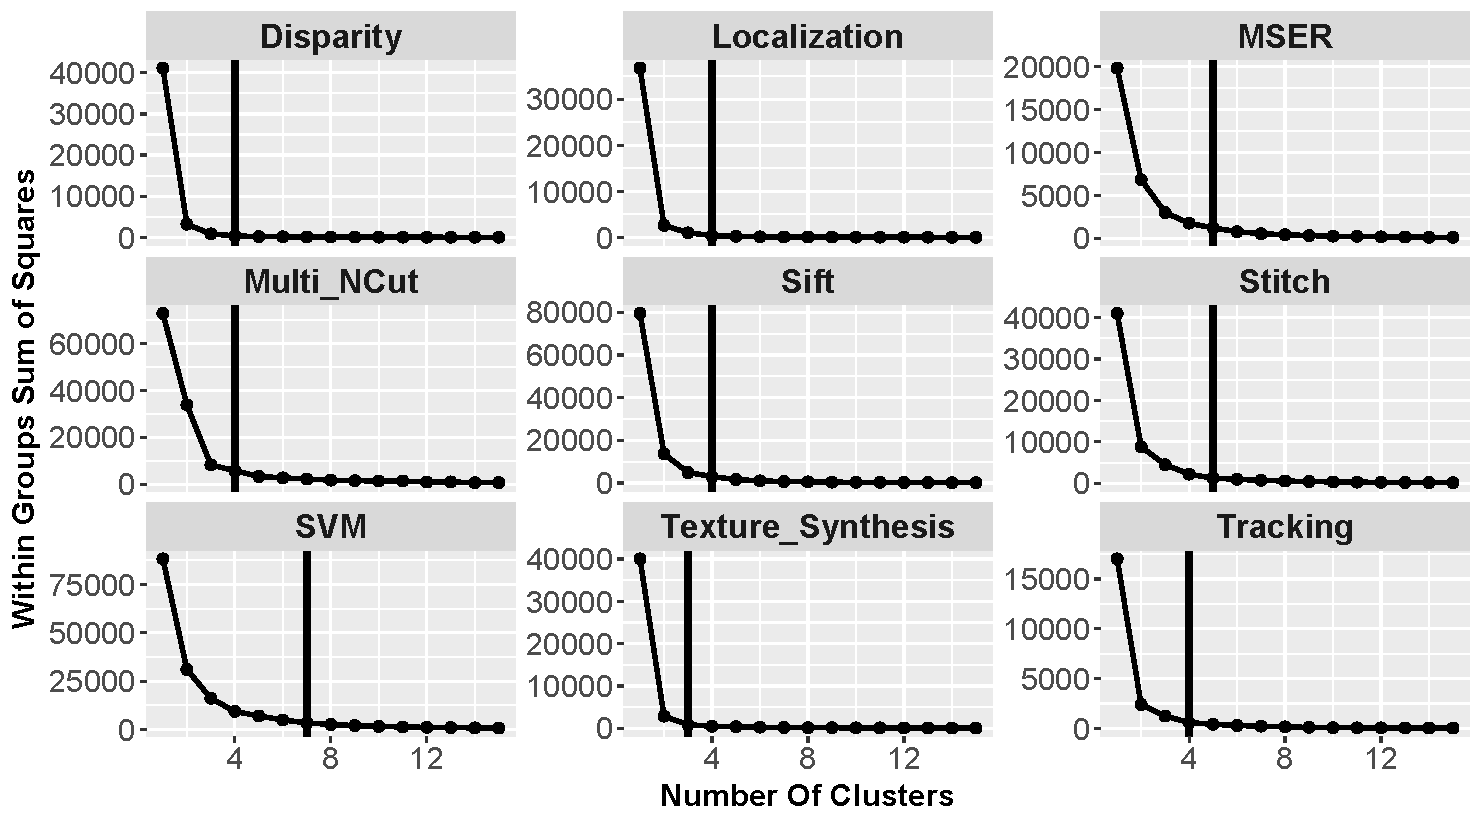
\includegraphics[width=1\textwidth]{cases-paper/graphics/Exploration/SSE_final.pdf}
    \caption{Sum of Square Errors given a number of k-means clusters for each of the benchmarks. The vertical line represents the number of clusters chosen for phase analysis.}
    \label{fig:sse}
		\vspace{1em}
\end{figure}

In order to find the correct number of clusters the Sum of Square Errors (SSE) is plotted for a given cluster size from 1 to 15 seen in Figure~\ref{fig:sse} and the optimal cluster is defined as the elbow in the plot~\cite{everitCluster2001}.
Applying a kMeans clustering to the IPCs of each application to determine phases is preferred to determining phases of an application by reading the source code phases.
This is because different source code passes may have the same IPC performance, and thus will ultimately belong to the same phase when considering core composition.
For example, the benchmark \bm{MSER}'s source code has 7 distinct passes, yet the kMeans clustering shows some of these passes result in the same performance, which can be visualised in Figure~\ref{fig:sxt}.
This kMeans clustering process is only done for the purpose of exploring this set of benchmarks.

\begin{figure}[t]
    \centering
    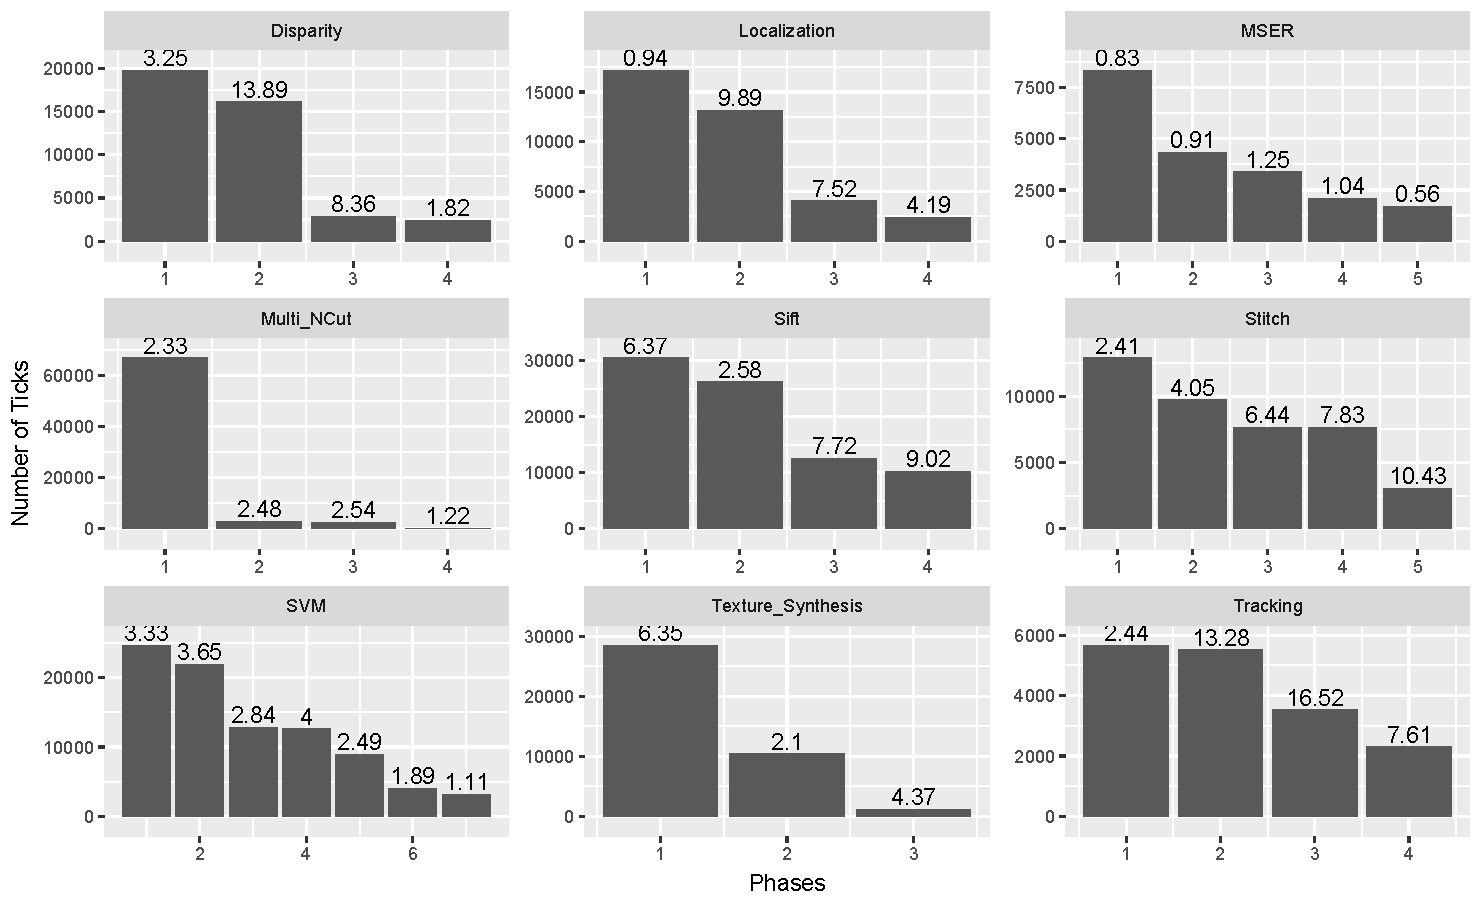
\includegraphics[width=1\textwidth]{cases-paper/graphics/Exploration/clusters4.pdf}
    \caption{Number of phases determined for each benchmark using kMeans clustering and their distribution. The number above each phase represents the average observed IPC.}
    \label{fig:clust}
		\vspace{1em}
\end{figure}

Figure~\ref{fig:clust} shows the number of clusters for each benchmark and the number of times a tick in each cluster occurs throughout the execution of the program and the average IPC observed for each cluster.
The frequency of a cluster is counted by how many ticks in the program are part of that specific phase.
The data can be corroborated with the information found in Figure~\ref{fig:sxt}.
For example, benchmark \bm{Multi\_NCut} features one phase covering over 80\% of the total execution, whereas for \bm{MSER}, the two dominant phases have very similar IPC values.
This means that it will be impossible to obtain any kind of performance improvements through dynamic reconfiguration due to the fact that there is little opportunity to switch the size of the composition.
For all the other benchmarks, they each have at least two dominant phases.
Since each phase is a cluster of similar IPC values, having two or more clusters will result in a higher chance of benefiting from dynamic core composition.

\begin{figure}[t]
    \centering
    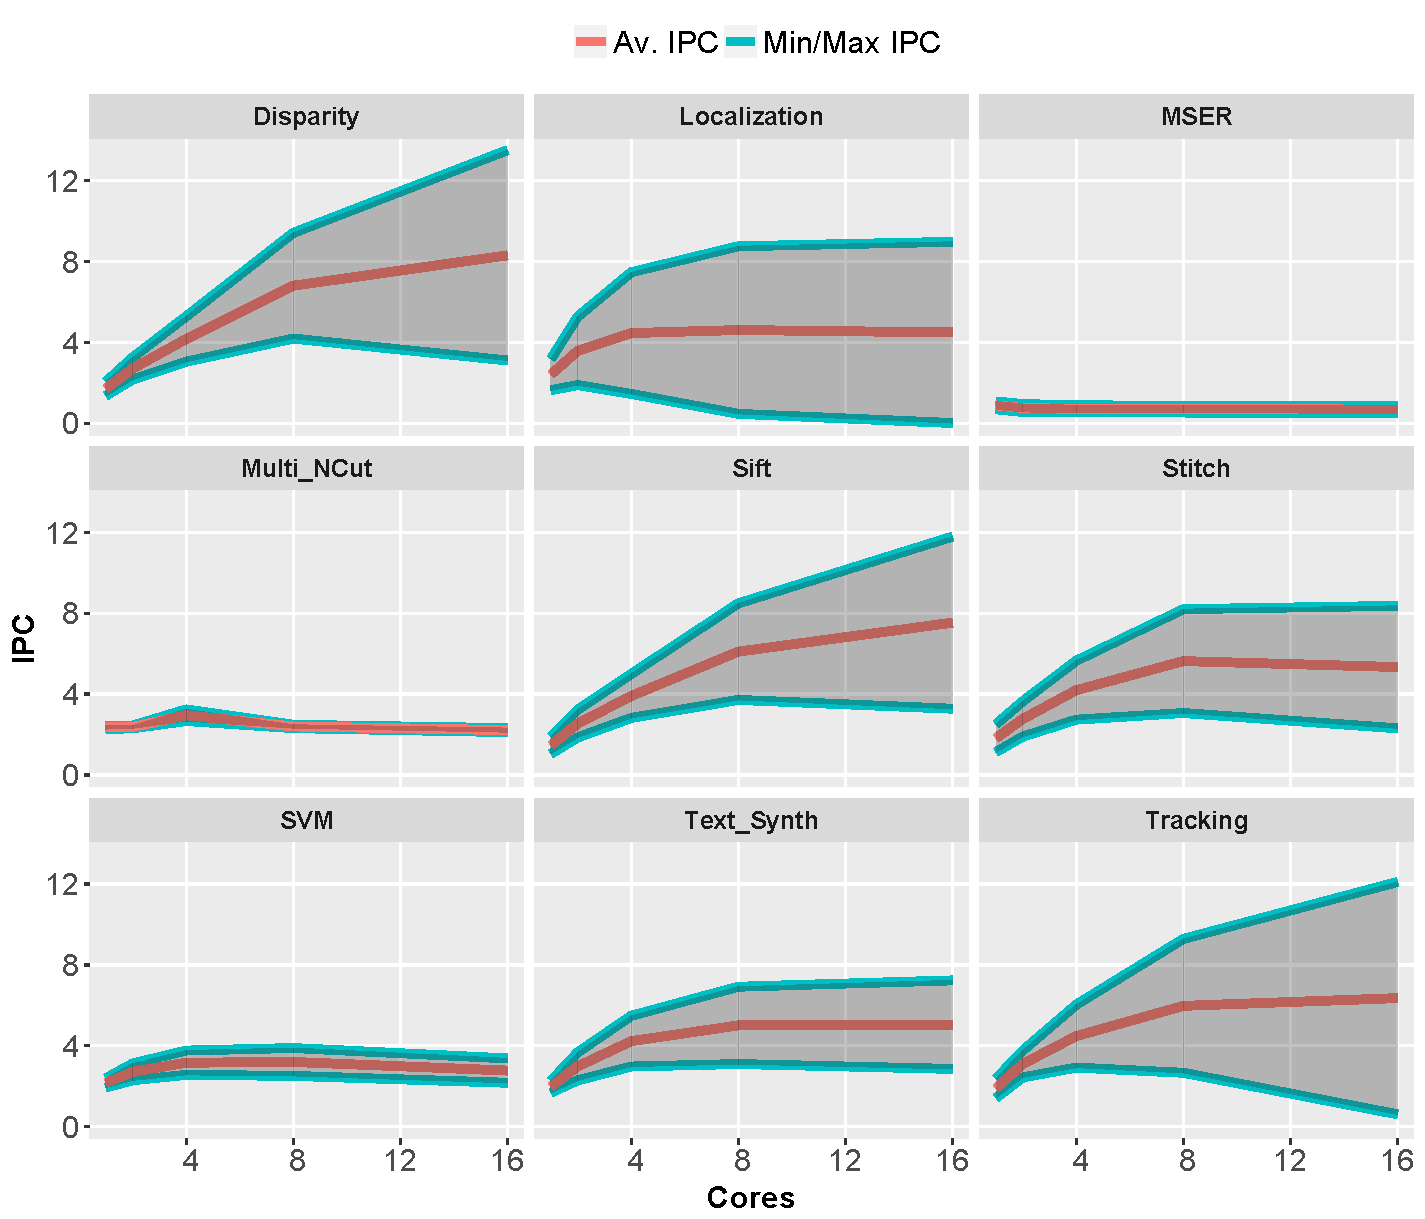
\includegraphics[width=1\textwidth]{cases-paper/graphics/Exploration/stddev3.pdf}
    \caption{Comparing average, minimum and maximum IPC for each SD-VBS benchmark using composition size of 16.}
    \label{fig:stddev}
		\vspace{5mm}
\end{figure}

\begin{figure}[t]
    \centering
    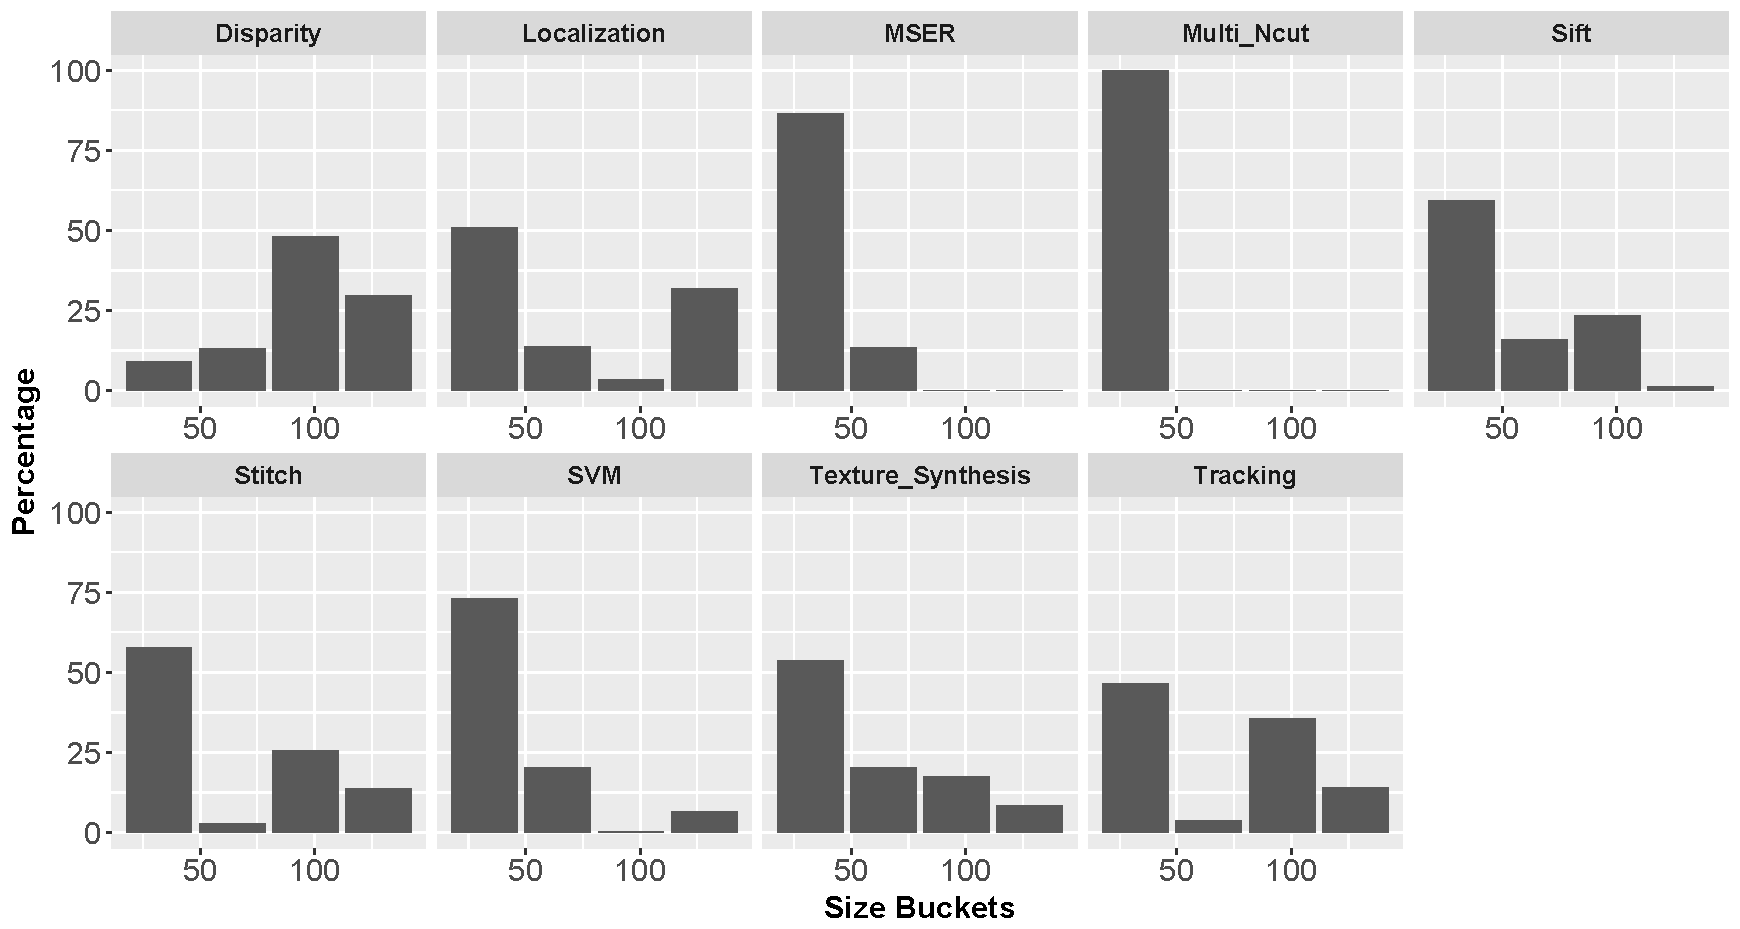
\includegraphics[width=1\textwidth]{cases-paper/graphics/Exploration/SizeBuckets.pdf}
	\vspace{-1em}
    \caption{Distribution of block sizes for each benchmark. The sizes are clustered in buckets equivalent to number of lanes occupied.}
    \label{fig:block_sizes}
	\vspace{5mm}
\end{figure}

\subsection{Static Ahead-of-Time Core composition Exploration}

In this chapter, Static Core composition defines a processor configuration that is determined ahead of time and does not change once it has been set.
Figure~\ref{fig:stddev} shows how the average Instructions Per Cycle (IPC) changes as the size of a core composition is increased, going in powers of 2 from 1 to 16 fused cores.
It can be seen that, for most benchmarks, fusing more cores provides an increase in IPC performance.
Benchmarks \bm{Disparity}, \bm{Localization}, \bm{Sift}, \bm{Stitch}, \bm{Texture Synthesis} and \bm{Tracking} all at least observe a speedup of 2x when using core composition.

However increasing the size of a composition is not always beneficial as can be seen in benchmarks \bm{Localization}, \bm{MSER}, \bm{Multi\_NCut}, \bm{Stich}, and \bm{SVM}.
For benchmarks \bm{Localization} and \bm{Stitch} the performance increases when fusing up to 8 cores, whereas \bm{MSER} and \bm{Multi\_NCut} never benefit from core composition.
These benchmarks may not see a reduction in performance on 16 cores due to the increase in network traffic, which will make the largest core composition size slower than 8 cores.
To summarise, when cores are fused, register files, caches and LSQs are shared, which means that cores must communicate via the network to send register or memory requests to other cores when the data they required is not stored locally.
Thus, having a higher number of cores composed will put pressure on the network.
Referring back to Figures~\ref{fig:sxt} and~\ref{fig:clust}, \bm{MSER} and \bm{Multi\_NCut} feature one dominating long phase with a very low IPC, and thus fusing cores cannot improve performance.

Figure~\ref{fig:stddev} also shows the variation of the IPC for each given composition size represented by the greyed out areas.
For example, running the \bm{Disparity} benchmark on a composition of 16 cores, it can be observed that an average IPC of 8.3.
The variation for 16 cores shows that the performance can drop down to 2.5.
An IPC of 2.5 when using 16 cores is very inefficient as this represents 0.1 of an instruction per cycle for each core and this performance can be achieved by using smaller core compositions.
Using a composition of size 4 for the \bm{Disparity} benchmark an average of 4.1 with a standard deviation of 1.2 is achieved.
Thus, if the composition could change size, there is a possibility that this could reduce the overall energy consumption of the system by switching from 16 to 4.

Figure~\ref{fig:block_sizes} shows the distribution of block-sizes for each of the benchmarks.
As two blocks cannot occupy the same lane, which is a segment of the instruction window (see Chapter~\ref{chp:Background}), the block sizes are clustered into groups which represent however many lanes will be occupied (one lane may execute a block of up to 32 instructions).
Using the information discussed in Section~\ref{sec:lim_study}, the size of blocks is a determining factor of whether or not a program may benefit from core composition.

Figure~\ref{fig:block_sizes} helps explain why benchmarks \bm{MSER} and \bm{Multi\_NCut} do not perform any better with core-composition.
For both cases, not only do they have a single detected phase, but both are predominantly formed of blocks that will occupy a single lane.
In fact, the most frequent block in \bm{MSER}, comprising 21\% the total executed blocks are comprised of only 8 instructions, whilst 31\% of \bm{Multi\_NCut}'s blocks are of 28 instructions.
Having such small blocks will always increase both the \textit{SynchronisationCost} and the branch-prediction requirements.

For \bm{MSER}, the fact that an important percentage of blocks are only 8 instructions long signifies that the overhead of fetching enough blocks for a large core-composition and the synchronisation cost for committing them outweighs executing the blocks on a single core.
The reason there is no degradation of performance is due to the fact that when fusing a high number of cores, if the overhead of fetching the blocks outweighs the time required to execute then a core will not submit a block address to be fetched by another core in the composition.
In this case, multiple cores may be composed, but only a single one is executing any code.
For example, fusing 16 cores and executing \bm{MSER} may in fact result in a single core being used due to it executing blocks faster than it being able to dispatch the blocks to a next core.
Hence, in this case, \bm{MSER} would be wasting a lot of energy trying to use 16 cores in a composition, whilst effectively only executing on a single core. 
This explains the lack of scaling for these two benchmarks.
The source code of \bm{MSER} and \bm{Multi\_NCut} is explored later on, to demonstrate how such small blocks are generated and why it cannot be improved.

Overall, most benchmarks that benefit from large compositions will also be met with an important difference in IPC performance.
The high difference in IPC performance is evidence of performance phases found in each application which are likely to benefit from dynamic adaptation.

%Need a better name for this
\subsection{Analysis of MSER and Multi\_NCut}

\begin{table}[t]
  \small
  \centering
 \begin{tabular} { | l | l | l | l | l | }
 \hline
   \cellcolor[gray]{0.7}Disparity & \cellcolor[gray]{0.7} Localization& \cellcolor[gray]{0.7} MSER& \cellcolor[gray]{0.7} Multi\_NCut& \cellcolor[gray]{0.7} Sift\\ \hline
	98\%  & 95\% & 85\%  & 100\%& 99\%\\ \hline
	 \cellcolor[gray]{0.7} Stitch & \cellcolor[gray]{0.7} SVM & \cellcolor[gray]{0.7} Text. Synth & \cellcolor[gray]{0.7} Tracking&\\ \hline
	  95\%& 93\%& 98\%& 98 \%&\\ \hline
	\end{tabular}
  \caption{Branch prediction accuracy in percentage for each of the benchmarks.}\label{tab:sd-vbsbpred}
  \vspace{1em}
\end{table}

As previously mentioned, both \bm{MSER} and \bm{Multi\_NCut} do not benefit from core-composition during their predominant phases.
This subsection focuses on understanding why this is the case and explores the code that represent the main phases of both of these applications to underline where the problems arise.
%Other code snipets from other SD-VBS benchmarks are also explored to demonstrate examples of code that perform well on core-compositions.

\lstset{
	backgroundcolor=\color{lbcolor},
	tabsize=2,
	rulecolor=,
	language=matlab,
        basicstyle=\tiny,
        upquote=true,
        aboveskip={1\baselineskip},
        columns=fixed,
        showstringspaces=false,
        extendedchars=true,
        breaklines=true,
        prebreak = \raisebox{0ex}[0ex][0ex]{\ensuremath{\hookleftarrow}},
        frame=single,
        showtabs=false,
        showspaces=false,
        showstringspaces=false,
        identifierstyle=\ttfamily,
        keywordstyle=\color[rgb]{0,0,1},
        commentstyle=\color[rgb]{0.133,0.545,0.133},
        stringstyle=\color[rgb]{0.627,0.126,0.941},
		numbers=left,
}

\paragraph*{MSER}
\bm{MSER} has five IPC phases according to Figure~\ref{fig:clust}; the two dominant phases represent the computation of the extremal regions tree.
As seen in Figure~\ref{fig:block_sizes}, the majority of the blocks in MSER are 8 instructions long, meaning that core-compositions will have to load the maximum amount of blocks (4 in this thesis) to fill each core.
The majority of \bm{MSER} is composed of tightly knit loops.
For example Listing~\ref{lst:mser-ex} shows two loops found in \bm{MSER's} main phase.
The rest of the source code of this phase can be found in the Appendix with Listing~\ref{lsting:mser}.
The while loops from the listing, alongside other while loops found in the phase (lines 36-39, 40-42 and 71-75) never run for more than a few iterations.
Due to the fact that these loops have small bodies, the fact that they do not run for many iterations would not make them candidates for unrolling.

\begin{figure}[t]
\lstset{language=C,numbersep=4pt}
\begin{center}
\begin{lstlisting}[firstnumber=27]
while( forest_pt[nrindex].shortcut != nrindex ) {          
	sref(visited_pt, nvisited++) = nrindex ;
	nrindex = forest_pt[nrindex].shortcut ;
}      
while( nvisited-- ) {
	forest_pt [ sref(visited_pt,nvisited) ] .shortcut = nrindex ;
}
\end{lstlisting}
\end{center}
\vspace{-1em}
\captionof{lstlisting}{Example of MSER loops (lines 27-30, 31-33).}
\label{lst:mser-ex}\vspace{1em}
\vspace{-3em}
\lstset{language=C,numbersep=4pt}
\begin{center}
\begin{lstlisting}[firstnumber=17]
for(k=0; k<rows; k++) {
        for(i=0; i<cols; i++) {
            float localMax = subsref(in,k,i);
            int localIndex = i;
            subsref(ind,k,i) = i;
            for(j=0; j<cols; j++) {
                if(localMax < subsref(in,k,j)) {
                    subsref(ind,k,i) = j;
                    localMax = subsref(in,k,j);
                    localIndex = j;
                }
            }
            subsref(in,k,localIndex) = 0;
        }
}
\end{lstlisting}
\end{center}
\vspace{-1em}
\captionof{lstlisting}{Main loop of Multi\_NCut.}
\label{lst:multi_loop}
\vspace{1em}
\end{figure}

It's also important to note that the average branch-prediction accuracy of \bm{MSER} is 85\%, as shown in Table~\ref{tab:sd-vbsbpred}.
Recalling Figure~\ref{fig:req_pred} and the fact that the average block size of \bm{MSER} is under 32 instructions, this means that no composition can be efficiently used.
Some speedup can still be obtained, as cores in a composition do not need to have the instruction window full to be able to obtain performance improvements.
However these improvements are minor, and come at a high energy cost.

To get performance out of \bm{MSER}, this major phase would have to be re-written to use fewer while loops with complex termination conditions so that larger blocks can be extracted.
Even with compiler optimisations, due to the fact that the loops are never executing for a long time, and their bodies are small and hard to unroll, it will be difficult to get performance improvements using core composition.

\paragraph*{Multi-NCut}

\bm{Multi\_NCut} is faced with a similar situation to \bm{MSER}.
Figure~\ref{fig:block_sizes} shows that once again, the majority of the blocks are less than 32 instructions long, in fact, over 50\% of the blocks are of 12 instructions or less.
Table~\ref{tab:sd-vbsbpred} shows that the branch prediction is always correct, yet, with blocks this small, the synchronisation cost of executing the blocks on large compositions outdoes any benefit that can be obtained via core-composition.
Listing~\ref{lst:multi_loop} shows the main loop of \bm{Multi\_NCut}; the rest of the source code can be found in Listing~\ref{lsting:multi}.%Listing~\ref{lsting:multi} in the Apendix shows the source code of the main phase of \bm{Multi\_NCut}, the main loop found at lines 17 to 31, also found in Listing~\ref{lst:multi_loop}.
Once again, this loop cannot be efficiently unrolled as the if statement can only be turned into a single hyperblock once.
For \bm{Multi\_NCut} the problem is that the blocks are too small which will cause the overhead of dispatching multiple blocks across a core-composition inefficient.
This is why the benchmark does not perform significantly better with core-composition without a high increase in energy consumption.


Overall, both benchmarks demonstrate that some loops cannot be adapted to benefit from core-composition.
This is especially true of while loops that cannot be converted into more traditional for loops.
Due to the small size of these loops, the overhead of dispatching multiple blocks over multiple cores outweighs the performance benefits.
